\section{Homogeneous flows}\label{homogeneous-flows}

\begin{figure}
\centering
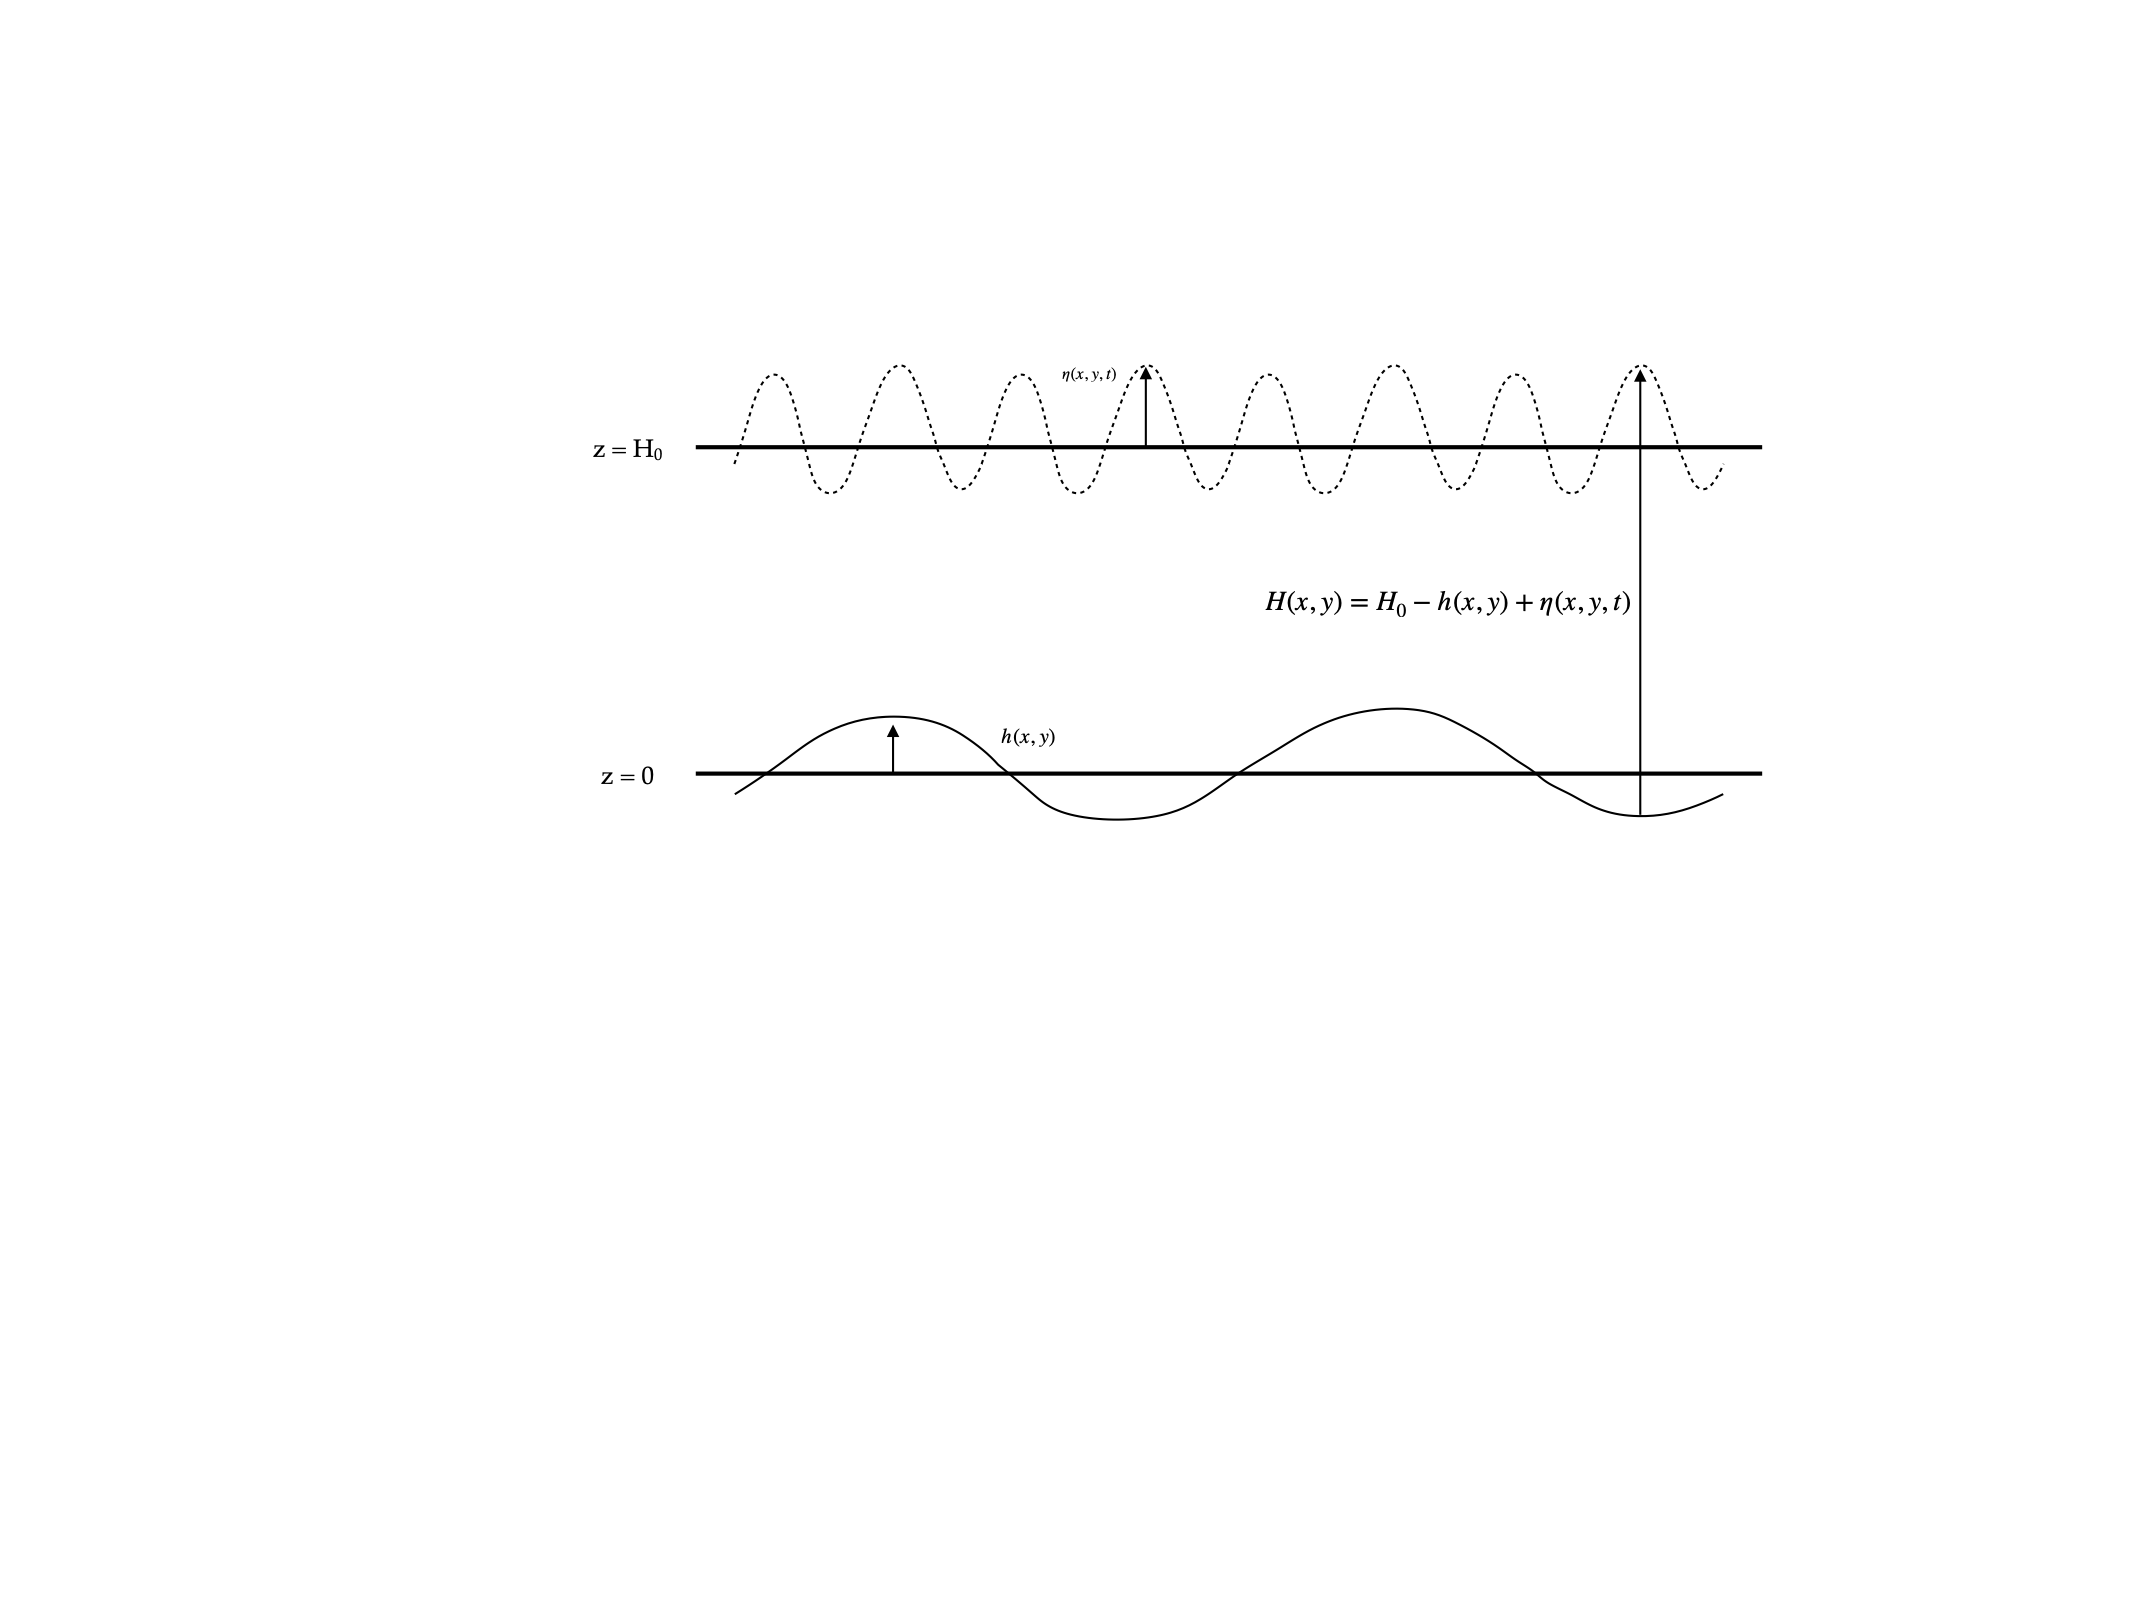
\includegraphics[width = .9 \textwidth]{./figs/GD/shw.png}
\caption{}
\label{}
\end{figure}


The motion of the atmosphere is most appropriately described by
three-dimensional equations that describes the horizontal and vertical
motion of the fluid, however a lot can be understood by considering a
simpler system that consider the motion of a free surface of a inviscid,
homogeneous and incompressible fluid. These equations are variously
referred to as one-level primitive equations or the shallow water
equation.

The system is described in Fig. \texttt{fig:4}. It is an homogenous
layer of fluid covering the entire spherical planet. We have included a
bottom topography \(h(x,y)\) and a deformation of the free surface
\(\eta(x,y)\). The convention is such positive deformation of the
surface are increasing the depth of the fluid, whereas positive
deformation of the bottom are decreasing it.

We have introduced here cartesian coordinates \((x,y)\) such that
\(dx \approx a \cos\theta d \lambda\) and \(dy \approx a d\theta\), we
will also define \(f= 2\Omega \sin\theta\), then the incompressible
equations of motion can be written as

\[
\begin{aligned}
\frac{\partial u}{\partial t} &= -u \frac{\partial u}{\partial x} -v \frac{\partial u}{\partial y} + f v -\frac{1}{\rho}\frac{\partial p}{\partial x} \\
\frac{\partial v}{\partial t} &= -u \frac{\partial v}{\partial x} -v \frac{\partial v}{\partial y} - f u -\frac{1}{\rho}\frac{\partial p}{\partial y}  \\
\frac{\partial w}{\partial t} &= -u \frac{\partial w}{\partial x} -v \frac{\partial w}{\partial y} + g -\frac{1}{\rho}\frac{\partial p}{\partial z}  \\
&\frac{\partial u}{\partial x} + \frac{\partial v}{\partial y} + \frac{\partial w}{\partial z} = 0
\end{aligned}
\]

If the aspect ratio \(\delta \approx H/L\) is small then hydrostatic
balance is maintained to order \(\delta^2\) and so

\[\frac{\partial p}{\partial z} = - \rho g + O(\delta^2)\]

because the density is constant we can integrate it from 0 to \(z\) and
get

\[p = -\rho g (H_0+ \eta -z) + p_0\]

where we have used the boundary condition at the top
\(p(x,y,H_0 +\eta) = p_0\).

The horizontal pressure gradients are independent of \(z\)

\[\begin{aligned}
\frac{\partial p}{\partial x} = \rho g \frac{\partial \eta}{\partial x}\\
\frac{\partial p}{\partial y} = \rho g \frac{\partial \eta}{\partial y}
\end{aligned}\]

because the horizontal accelerations are independent of z, than also the
velocities are independent of z, if they are so at the beginning. This
is in fact a consequence of the Taylor-Proudman theorem applied to a
homogeneous fluid. We can then write the horizontal momentum equations

\[\begin{aligned}
\frac{\partial u}{\partial t} &= -u \frac{\partial u}{\partial x} -v \frac{\partial u}{\partial y} + f v -g\frac{\partial \eta}{\partial x} \\
\frac{\partial v}{\partial t} &= -u \frac{\partial v}{\partial x} -v \frac{\partial v}{\partial y} - f u -g\frac{\partial \eta}{\partial y}  \\
\end{aligned}\]

Because \(u\) and \(v\) are independent of \(z\) allows us to integrate
vertically the divergence equation from the surface \(h(x,y)\) to an
height \(z\)

\[w(x,y,z,t) = -z\left(\frac{\partial u}{\partial x} + \frac{\partial v}{\partial y}\right) + \omega(x,y,t)\]

The kinematic condition for the bottom can be written as

\[\frac{D }{Dt}{(z-h)} = 0\]

or

\[w(x,y,h,t) =  u\frac{\partial h}{\partial x} + v\frac{\partial h}{\partial y}\]

so the function \(\omega\) is

\[\omega(x,y,t) = u\frac{\partial h}{\partial x} + v\frac{\partial h}{\partial y} + h \left(\frac{\partial u}{\partial x} + \frac{\partial v}{\partial y}\right)\]

then the vertical velocity can be written as

\[w(x,y,z,t) = (h-z)\left(\frac{\partial u}{\partial x} + \frac{\partial v}{\partial y}\right) + u\frac{\partial h}{\partial x} + v\frac{\partial h}{\partial y}\]

Using now the kinematic boundary condition at the top (\(z=H_0+\eta\))

\[w(x,y,H_0+\eta,t) = \left(\frac{\partial }{\partial t} + u\frac{\partial }{\partial x} + v\frac{\partial }{\partial y}\right)(H_0+\eta)\]

combining the last two equation we get an equation for the height

\[\frac{\partial \eta}{\partial t} + \frac{\partial }{\partial x}(H_0+\eta -h)u + \frac{\partial }{\partial y}(H_0+\eta -h)v = 0\]

and so we can now write the complete equations, introducing the total
depth of the fluid \(H=H_0+\eta -h\):

\[\begin{aligned}
\frac{\partial u}{\partial t} &= -u \frac{\partial u}{\partial x} -v \frac{\partial u}{\partial y} + f v -g\frac{\partial H}{\partial x} \\
\frac{\partial v}{\partial t} &= -u \frac{\partial v}{\partial x} -v \frac{\partial v}{\partial y} - f u -g\frac{\partial H}{\partial y}  \\
\frac{\partial H}{\partial t} &= - \frac{\partial (u H)}{\partial x} - \frac{\partial (v H)}{\partial y} \\
\end{aligned}\]

\subsection{The shallow equation in spherical
coordinates}\label{the-shallow-equation-in-spherical-coordinates}

The equation in spherical coordinates describing such a system, with a
flat bottom (\(h(x,y) =0\)), are

\[\begin{aligned}
\frac{\partial u}{\partial t}  +\frac{u}{a \cos\theta} \frac{\partial u}{\partial \lambda} +\frac{v}{a} \frac{\partial u}{\partial \theta} +\frac{1}{a} u v \tan\theta- 2\Omega\sin\theta  v &= -\frac{1}{a \cos\theta}\frac{\partial \eta}{\partial \lambda} \\
\frac{\partial v}{\partial t}  +\frac{u}{a \cos\theta} \frac{\partial v}{\partial \lambda} +\frac{v}{a} \frac{\partial v}{\partial \theta}  +\frac{1}{a} u^2 \tan\theta + 2\Omega\sin\theta u &= -\frac{1}{a}\frac{\partial \eta}{\partial \theta} \label{uvsphfluxform} \\
\frac{\partial \eta}{\partial t} +\frac{1}{a \cos^2\theta}\left[\frac{\partial }{\partial \lambda}(u\cos\theta \eta) +\cos\theta\frac{\partial }{\partial \theta}(v\cos\theta \eta) \right] &= \\
-  \frac{H_0}{a \cos^2\theta} \left[\cos\theta \frac{\partial }{\partial \theta} (v \cos\theta ) + \frac{\partial u\cos\theta}{\partial \lambda}\right]
\end{aligned}\]

and the total height of the fluid is \(H_0+\eta\) where \(H_0\) is a
global constant. The quantity in bracket on the right hand side of the
free surface equation is the divergence in spherical coordinates

\[D=\frac{1}{a \cos^2\theta}\left[\cos\theta \frac{\partial }{\partial \theta} (v \cos\theta ) + \frac{\partial }{\partial \lambda}(u\cos\theta)\right]\]

and together with the relative vorticity

\[\zeta=\frac{1}{a \cos^2\theta}\left[ \frac{\partial }{\partial \lambda} (v \cos\theta ) - \cos\theta\frac{\partial }{\partial \theta}(u\cos\theta)\right]\]

can be used to write the equations in terms of vorticity and divergence.
Considering that the velocities can be expressed in terms of a
streamfunction and of a velocity potential

\[\begin{aligned}
u &= -\frac{1}{a}\frac{\partial \psi}{\partial \theta} + \frac{1}{a\cos\theta}\frac{\partial \chi}{\partial \lambda}\\
v &= \frac{1}{a\cos\theta}\frac{\partial \psi}{\partial \lambda} + \frac{1}{a}\frac{\partial \chi}{\partial \theta}
\end{aligned}\]

it is simple to show that

\[\zeta = \nabla^2 \psi \qquad D = \nabla^2\chi\]

the momentum equations can be recast in terms of vorticity and
divergence, two scalar quantities as

\[\begin{aligned}
\frac{\partial \zeta}{\partial t} &= -\frac{1}{a \cos^2\theta}\left[ \frac{\partial }{\partial \lambda}(U\zeta) + \cos\theta\frac{\partial }{\partial \theta}(V\zeta)\right] - 2 \Omega\left(\sin\theta D +\frac{V}{a}\right)\\
\frac{\partial D}{\partial t} &= \frac{1}{a \cos^2\theta}\left[ \frac{\partial }{\partial \lambda}(V\zeta) - \cos\theta\frac{\partial }{\partial \theta}(U\zeta)\right] + 2 \Omega\left(\sin\theta \zeta -\frac{U}{a}\right) -\nabla^2\left( \frac{U^2+V^2}{2 \cos^2\theta} + \eta\right)\\
\frac{\partial \eta}{\partial t} &= -\frac{1}{a \cos^2\theta}\left[\frac{\partial }{\partial \lambda}(U \eta) + \cos\theta\frac{\partial }{\partial \theta}(V \eta)\right]  - H_0 D
\end{aligned}\]

where \(U = u \cos\theta, \,\, V = v \cos\theta\).

\subsection{The incompressible
equations}\label{the-incompressible-equations}

If we assume that the free surface do not move, \(\eta=0\), then the
continuity equations implies that the flow has zero divergence, D = 0,
and the only equation left is the vorticity equation in more simplified
form

\[\frac{\partial \zeta}{\partial t} = -\frac{1}{a \cos^2\theta}\left[ \frac{\partial }{\partial \lambda}(U\zeta) + \cos\theta\frac{\partial }{\partial \theta}(V\zeta)\right] - 2 \Omega\frac{V}{a}\]

and the advection terms also simplifies using the zero divergence

\[\frac{\partial \zeta}{\partial t} = -\frac{u}{a \cos\theta} \frac{\partial \zeta}{\partial \lambda} -\frac{v}{a} \frac{\partial \zeta}{\partial \theta}- 2 \Omega\frac{V}{a}\]

or

\[\frac{D }{Dt}(\zeta + f) =0\]

\subsection{\texorpdfstring{The vorticity equation on the
\(\beta\)-plane}{The vorticity equation on the \textbackslash beta-plane}}\label{the-vorticity-equation-on-the-beta-plane}

The spherical geometry maybe cumbersome without adding much the
conceptual discussions, so it may be convenient to introduce cartesian
coordinates \((x,y)\) such that \(dx \approx a \cos\theta d \lambda\)
and \(dy \approx a d\theta\), we will also define
\(f= 2\Omega \sin\theta\), then we obtain equation formally identical to
the Cartesian equation described previously

\[\begin{aligned}
\frac{\partial u}{\partial t} &= -u \frac{\partial u}{\partial x} -v \frac{\partial u}{\partial y} + f v -g\frac{\partial \eta}{\partial x} \\
\frac{\partial v}{\partial t} &= -u \frac{\partial v}{\partial x} -v \frac{\partial v}{\partial y} - f u -g\frac{\partial \eta}{\partial y} \\
&\frac{\partial u}{\partial x}+\frac{\partial v}{\partial y} = 0 \\
\end{aligned}\]

where we have kept the pressure terms, though they are zero in this case
( h is a constant) as a placeholder. In vector notation (all vectors are
two-dimensional)

\[\frac{\partial \mathbf{v}}{\partial t} = - (\mathbf{v} \cdot \nabla)\mathbf{v} - f(\hat{k}\times \mathbf{v}) - \nabla \eta\]

using the vector identity

\[\frac{1}{2}\nabla(A\cdot A) = (A \cdot\nabla)A + A\times(\nabla\times A)\]

or

\[\frac{1}{2}\nabla(\mathbf{v}\cdot \mathbf{v}) = (\mathbf{v} \cdot\nabla)\mathbf{v} + \mathbf{v}\times(\nabla\times \mathbf{v})\]

so substituting in the equation

\[\frac{\partial \mathbf{v}}{\partial t} = -(\zeta + f) \hat{k}\times \mathbf{v} -\nabla(\eta+\frac{1}{2}|\mathbf{v}^2|)\]

(for 2-dimensional flows \(\nabla \times \mathbf{v} = \zeta \hat{k}\)).

and to express more clearly the components

\[\begin{aligned}
\frac{\partial u}{\partial t} &= (\zeta +f) v -\frac{\partial }{\partial x}(\eta+\frac{1}{2}|\mathbf{v}^2|)\\
\frac{\partial v}{\partial t} &= -(\zeta +f) u -\frac{\partial }{\partial y}(\eta+\frac{1}{2}|\mathbf{v}^2|)
\end{aligned}\]

By taking the curl of eq.(\texttt{Eq21}) we obtain an equation for the
vorticity

\[\begin{aligned}
\frac{\partial \zeta}{\partial t} &= -\frac{\partial }{\partial x}(\zeta +f) u -\frac{\partial }{\partial y}(\zeta +f) v  \\
&-\frac{\partial }{\partial x} \frac{\partial }{\partial y}(p+\frac{1}{2}|\mathbf{v}^2|) +\frac{\partial }{\partial y}\frac{\partial }{\partial x}(p+\frac{1}{2}|\mathbf{v}^2|) \\
&=  -\frac{\partial }{\partial x}(\zeta +f) u -\frac{\partial }{\partial y}(\zeta +f) v = -\mathbf{v}\cdot\nabla(\zeta +f)
\end{aligned}\]

where we have used the non divergence condition
\(\frac{\partial u}{\partial x}+\frac{\partial v}{\partial y}=0\) in the
last step. Once again, this is the equation for the conservation of
total vorticity where we can see that the relative vorticity is a sort
of additional Coriolis effect (or alternatively that the Coriolis term
is a source of vorticity).

\[\frac{D}{Dt}(\zeta +f)=0\]

\(f= 2\Omega \sin(\theta)\) is the Coriolis coefficient, that is the
vertical component of the Earth planetary vorticity. The fluid is
homogeneous, so there are no vertical velocities, it is independent of
the vertical coordinate \(z\) and so we can write

\[\frac{\partial \zeta}{\partial t} = - \mathbf{v} \cdot \nabla (\zeta +f) = -\mathbf{\nabla}\cdot(\mathbf{v}(\zeta+f) )= -\mathbf{v}\cdot\nabla \zeta - \beta v\]

where

\[\beta = \frac{1}{a} \frac{\partial f}{\partial \theta} = \frac{ 2 \Omega }{a}\cos \theta\]

This equation is still somewhat imprecise because we are mixing the
cartesian coordinates without a rigorous coordinate transformation. In
order to do that we have to recast Eq \texttt{ErtelBTP} on the
\(\beta\)-plane, As it often the case with approximations, it will be
found that we can stretch the range of validity of this assumption
somewhat and consider scales that are relatively larger with respect the
planet. This assumption is approximating the sphericity of the Earth
with a tangent plane at a latitude point \(\theta_0\), in this case the
cartesian coordinate become rigorous and the Coriolis factor \(f\) can
be approximated by a linear expression

\[f = \frac{ 2 \Omega }{a}\sin\theta= \frac{ 2 \Omega }{a}\left[ \sin\theta_0 + \cos\theta_0(\theta - \theta_0)\right] = f_0 + \beta y\]

The non-divergent barotropic vorticity equation can then be written as

\[\frac{\partial \zeta}{\partial t} = - u \frac{\partial \zeta}{\partial x} - v\frac{\partial \zeta}{\partial y} - \beta v\]

in the new coordinates \((x,y)\) for longitude and latitude, the
streamfunction and the vorticity then are

\[u=-\frac{\partial \psi}{\partial y}\qquad v=\frac{\partial \psi}{\partial x} \qquad
\zeta = \frac{\partial x}{\partial x} -\frac{\partial u}{\partial y}=\nabla^2\psi\]

introducing the Jacobian operator

\[J(A,B) = \frac{\partial A}{\partial x}\frac{\partial B}{\partial y} - \frac{\partial A}{\partial y}\frac{\partial B}{\partial x}\]

we obtain a single equation for the streamfunction

\[\frac{\partial }{\partial t}\nabla^2\psi  + J(\psi, \nabla^2\psi +f_0 + \beta y) = 0\]

\subsection{Accelerating the zonal flow}\label{accelerating-the-zonal-flow}

Averaging Eq \texttt{Eq21} results in a simpler equation for the
acceleration of the zonal wind \(u\)

\[\frac{\partial \bar{u}}{\partial t} = \overline{(\zeta+f) v}\]

and averaging the equation of the zonal momentum in flux form from Eq.
\texttt{uvfform}

\[\begin{aligned}
\frac{\partial u}{\partial t} &= -\frac{\partial }{\partial x}\frac{u^2}{2} -\frac{\partial }{\partial y}(u v) +f v -\frac{\partial p}{\partial x}\\
\frac{\partial \bar{u}}{\partial t} &= \overline{-\frac{\partial }{\partial x}\frac{u^2}{2}} -\overline{\frac{\partial }{\partial y}(u v)} +\overline{f v} -\overline{\frac{\partial p}{\partial x}}
\end{aligned}\]

the only surviving term is the second term that expresses correlations
between the component of the horizontal velocity. Because the zonal
averaging is acting only on the longitudes, the \(x\) coordinate, we can
look only at the nonlinear term. Expanding the term we have

\[\overline{u v} = \overline{(\bar{u}+u')(\bar{v}+v')} = \overline{\bar{u}\bar{v}+ \bar{u}v' + u'\bar{v}+ u'v'}\]

the only term that is not zero is last term, so
\(\overline{uv}=\overline{u'v'}\), the zonal mean of quadratic terms
involving the meridional velocity is depending only on the deviations
frok the zona mean itself.. And finally:

\[\frac{\partial \bar{u}}{\partial t} = -\frac{\partial }{\partial y}\overline{u'v'}\]

but applying the decomposition rule also to the vorticity this implies
that

\[\overline{\zeta'v'}=-\frac{\partial }{\partial y}\overline{u'v'}\]

This discussion shows that the acceleration of the zonal flow is due to
the gradient of meridional transport of eddy zonal momentum by the
deviations from the zonal means. The gradient is equivalent to the
meridional eddy transport of eddy vorticity.
